\documentclass[aspectratio=169,10pt]{beamer}
\usetheme{Madrid}
\usecolortheme{whale}
\usepackage{booktabs}
\usepackage{graphicx}
\usepackage{amsmath}
\usepackage{tikz}
\usetikzlibrary{arrows.meta,positioning,fit,backgrounds}
\setbeamertemplate{navigation symbols}{}
\setbeamerfont{footnote}{size=\tiny}
\definecolor{mu2eblue}{RGB}{0,51,102}
\setbeamercolor{title}{fg=white}

\title[Foils vs Flash]{Stopping-Target Foils vs Electron-Beam Flash}
\subtitle{Extra foils swing tracker flash per POT $3.1\times$ --- at no S/$\sqrt{B}$ cost}
\author{Y.\ Oksuzian}
\institute[Mu2e autoresearch]{Mu2e --- autoresearch / closed-loop Bayesian optimization}
\date{2026-07-24}

\begin{document}

\begin{frame}
\titlepage
\end{frame}

\begin{frame}{Result in one slide}
\begin{block}{}
Extra stopping-target foils are a \textbf{real lever on the electron-beam flash}:
tracker flash per POT varies \textbf{3.1$\times$} across the explored geometry,
at \textbf{no S/$\sqrt{B}$ cost}.
\end{block}
\vspace{0.5em}
\begin{itemize}
  \item \textbf{339 evals} from closed-loop Bayesian optimization map a clean Pareto front.
  \item \textbf{Champion} \texttt{ff11R00\_07} beats the deployed target on \emph{both} axes:
        S/$\sqrt{B}$ 3.31 vs 3.11, flash $-3\%$.
  \item The S/$\sqrt{B}$ ceiling (\textbf{3.90}) is \textbf{confirmed reproducible}; a dense
        basin scan found \texttt{BASIN01\_11} --- same 3.90 at \textbf{$-$5.8\% flash} vs the
        transplant (400-seed confirmed, $\sim$3.2$\sigma$).
\end{itemize}
\end{frame}

\begin{frame}{What we optimize}
\textbf{6-D extra-foil geometry}: up to 6 upstream and 6 downstream extra foils on the
pinned 37-foil base --- outer radius, half-thickness, and hole fraction, independently
up and down.
\vspace{1.5em}
\begin{center}
\small
\begin{tabular}{@{}p{0.42\textwidth} l p{0.30\textwidth}@{}}
\toprule
objective & direction & source \\
\midrule
S/$\sqrt{B}$ & \textbf{maximize} & Run1A CE significance \\
$e^-$ early-flash edep \textbf{per POT} in tracker & \textbf{minimize} & \texttt{elebeam\_flash}, DS-on \\
\bottomrule
\end{tabular}
\end{center}
\end{frame}

\begin{frame}{How the loop works}
\begin{center}
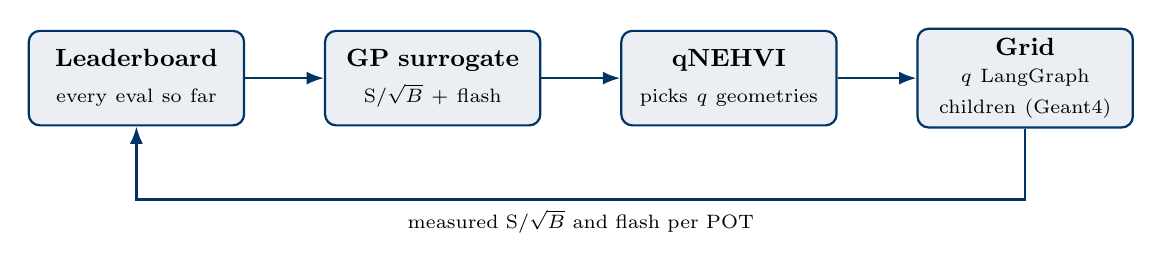
\begin{tikzpicture}[
  font=\small,
  box/.style={draw=mu2eblue, thick, rounded corners, fill=mu2eblue!8,
              text width=2.5cm, align=center, minimum height=1.2cm},
  arr/.style={-{Latex[length=2.2mm]}, thick, draw=mu2eblue}
]
\node[box] (lb) {\textbf{Leaderboard}\\[2pt]\scriptsize every eval so far};
\node[box, right=1.0cm of lb]  (gp)   {\textbf{GP surrogate}\\[2pt]\scriptsize S/$\sqrt{B}$ $+$ flash};
\node[box, right=1.0cm of gp]  (acq)  {\textbf{qNEHVI}\\[2pt]\scriptsize picks $q$ geometries};
\node[box, right=1.0cm of acq] (grid) {\textbf{Grid}\\[2pt]\scriptsize $q$ LangGraph\\children (Geant4)};

\draw[arr] (lb)  -- (gp);
\draw[arr] (gp)  -- (acq);
\draw[arr] (acq) -- (grid);

\draw[arr] (grid.south) -- ++(0,-0.9) coordinate (fb)
           -- node[below, font=\scriptsize] {measured S/$\sqrt{B}$ and flash per POT}
              (fb -| lb.south) -- (lb.south);
\end{tikzpicture}
\end{center}
\vspace{1em}
\footnotesize
$q$ geometries are in flight at once; each returns one measured row, and the surrogate
refits as rows land. Nothing reaches the leaderboard that was not actually simulated.
\end{frame}

\begin{frame}{Inside one evaluation}
\begin{center}
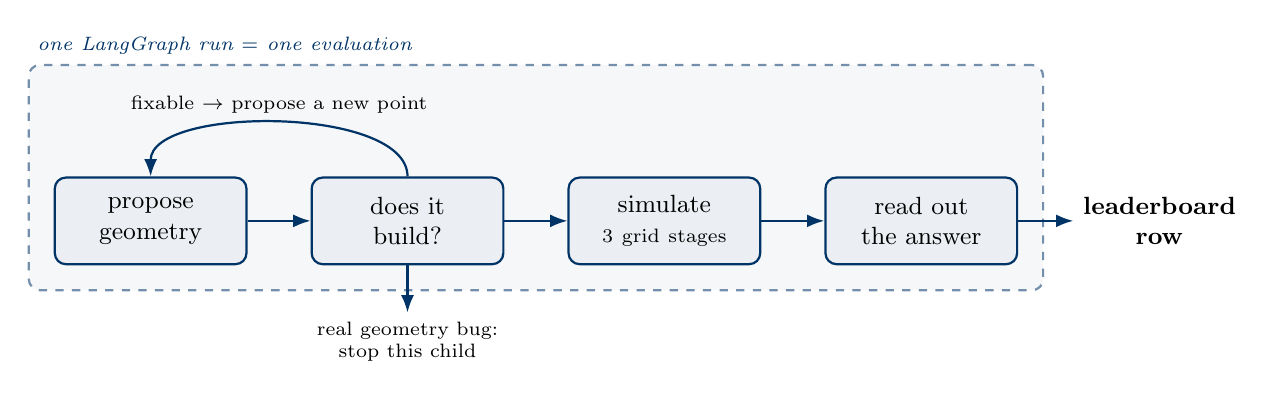
\begin{tikzpicture}[
  font=\small,
  box/.style={draw=mu2eblue, thick, rounded corners, fill=mu2eblue!8,
              text width=2.2cm, align=center, minimum height=1.1cm},
  arr/.style={-{Latex[length=2.2mm]}, thick, draw=mu2eblue}
]
\node[box] (prop) {propose\\geometry};
\node[box, right=0.8cm of prop] (pf)  {does it\\build?};
\node[box, right=0.8cm of pf]   (sim) {simulate\\\scriptsize 3 grid stages};
\node[box, right=0.8cm of sim]  (out) {read out\\the answer};
\node[right=0.7cm of out, align=center] (row) {\textbf{leaderboard}\\\textbf{row}};

\draw[arr] (prop) -- (pf);
\draw[arr] (pf)   -- (sim);
\draw[arr] (sim)  -- (out);
\draw[arr] (out)  -- (row);

\draw[arr] (pf.north) .. controls +(0,0.9) and +(0,0.9) ..
      node[above, font=\scriptsize] {fixable $\rightarrow$ propose a new point} (prop.north);

\node[below=0.6cm of pf, font=\scriptsize, align=center] (bug)
      {real geometry bug:\\stop this child};
\draw[arr] (pf.south) -- (bug);

% invisible anchor so the retry curve sits inside the LangGraph region
\node[above=1.05cm of pf, inner sep=0pt] (apex) {};
\begin{scope}[on background layer]
  \node[draw=mu2eblue!55, dashed, thick, rounded corners, inner sep=9pt,
        fill=mu2eblue!4, fit=(prop)(pf)(sim)(out)(apex)] (lg) {};
\end{scope}
\node[anchor=south west, font=\scriptsize\itshape, text=mu2eblue]
      at (lg.north west) {one LangGraph run $=$ one evaluation};
\end{tikzpicture}
\end{center}
\vspace{0.5em}
\begin{itemize}\scriptsize
  \item \textbf{LangGraph} is a small state-machine library: you declare \emph{nodes} (steps)
        and \emph{edges} (transitions); it runs them and saves the state after each.
  \item \textbf{We use it for exactly one job:} driving a single evaluation from proposal to
        leaderboard row --- the optimizer loop around it is plain Python.
  \item Saved state means a child that dies mid-chain \textbf{resumes} instead of re-submitting
        grid jobs.
  \item \textbf{Read out the answer} $=$ reduce the finished jobs' outputs to two numbers:
        CE ntuple $\rightarrow$ S/$\sqrt{B}$, tracker straw-gas energy $\rightarrow$ flash per POT.
  \item Any failed stage \textbf{halts the chain}: no row is ever written from partial results.
\end{itemize}
\end{frame}

\begin{frame}{The actual LangGraph topology}
\begin{columns}[T]
\begin{column}{0.44\textwidth}
\centering
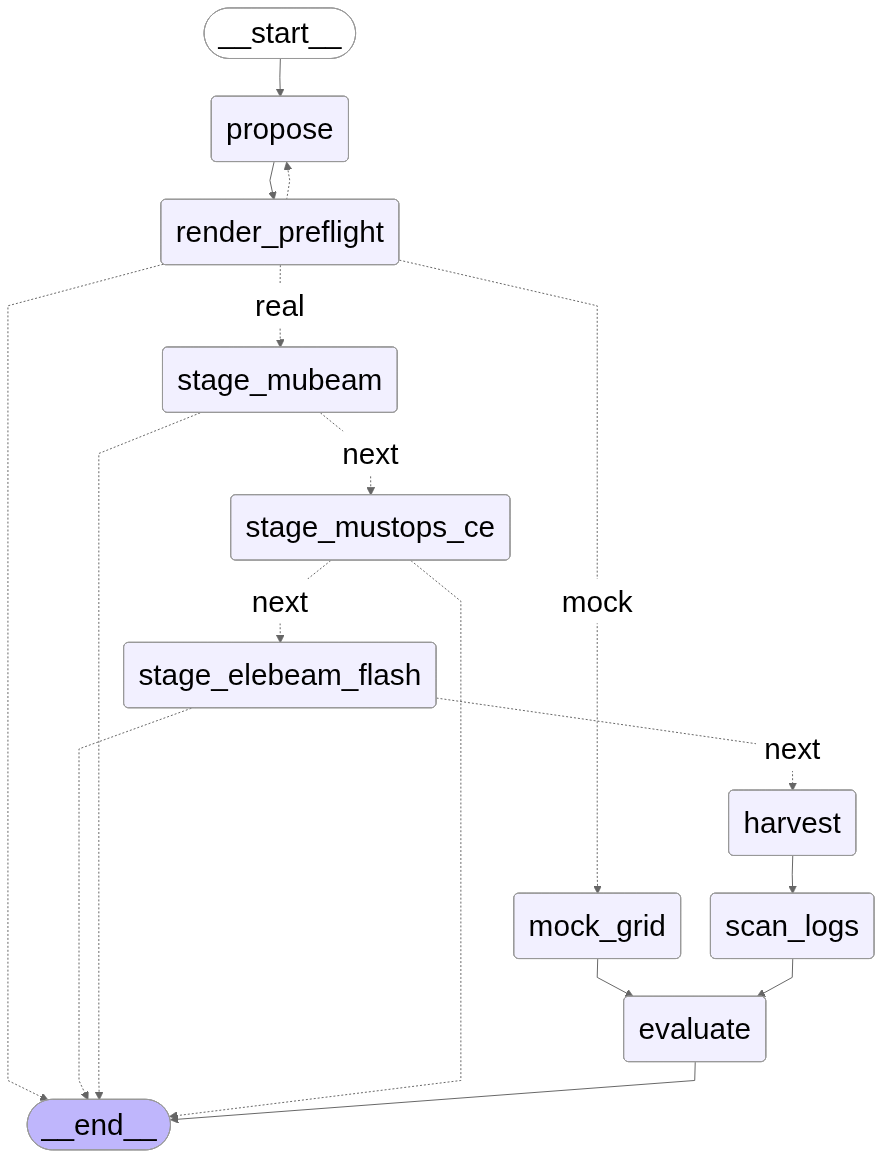
\includegraphics[height=0.80\textheight]{foilsflash_langgraph.png}
\end{column}
\begin{column}{0.54\textwidth}
\scriptsize
Generated from the running code --- \texttt{get\_graph().draw\_mermaid()}, foilsflash mode ---
so it cannot drift from what actually executes.
\vspace{0.8em}
\begin{itemize}\scriptsize
  \item \texttt{propose} / \texttt{render\_preflight} --- pick the point, write the geometry,
        cheap local Geant4 init check.
  \item \texttt{stage\_*} --- the three grid stages, in chain order.
  \item \texttt{harvest} / \texttt{scan\_logs} --- reduce the outputs to the two metrics, and
        refuse the row if the log scan finds physics-breaking patterns.
  \item \texttt{evaluate} --- append the leaderboard row.
  \item \textbf{Dotted} edges are conditional: the preflight retry, the per-stage fail-fast to
        \texttt{\_\_end\_\_}, and the \texttt{mock} path used by tests.
  \item \textbf{Control flow, not a timeline:} \texttt{stage\_elebeam\_flash} is last in the chain,
        but its jobs were submitted inside the \texttt{stage\_mubeam} node --- they ran during
        \texttt{stage\_mustops\_ce}, so the node only polls. The overlap is a side effect, not an edge.
\end{itemize}
\vspace{0.3em}
\hrule
\vspace{0.3em}
{\tiny
\textbf{Launch a campaign} ($q$ children, rolling):\\[2pt]
\texttt{AUTORESEARCH\_MODE=foilsflash \textbackslash}\\
\texttt{python -m graph.closed\_loop --mode foilsflash \textbackslash}\\
\texttt{\ \ --name-prefix foilsflash20 --picker hybrid \textbackslash}\\
\texttt{\ \ --q 5 --max-evals 10 --rolling}\\[5pt]
\textbf{One evaluation} (exactly the graph at left):\\[2pt]
\texttt{python -m graph.run --mode foilsflash --no-mock \textbackslash}\\
\texttt{\ \ --config-name ff20R00\_00 --x-point <6 values>}
}
\end{column}
\end{columns}
\end{frame}

\begin{frame}{How the machinery behaves}
\small
\begin{tabular}{@{}p{0.40\textwidth}p{0.56\textwidth}@{}}
\toprule
question & answer \\
\midrule
Where is LangGraph? &
One \emph{evaluation} $=$ one LangGraph run. The optimizer loop around it is plain Python. \\[3pt]

When does a stage pass? &
Quorum, not all jobs: \textbf{12/15} for \texttt{mubeam} and \texttt{mustops\_ce} (0.8),
\textbf{90/100} for \texttt{elebeam\_flash} (0.9). \\[3pt]

Does harvest start there? &
No --- it also waits for the \emph{outputs} to land on /pnfs. Jobs leave the queue minutes
before stage-out finishes. \\[3pt]

Does a failed stage retry? &
No. Preflight retries 3$\times$ (2 min, local); a stage has already spent $\sim$90 min of grid
--- it stops and a human looks. \\[3pt]

What ends a run early? &
Geometry that will not build, 3 failed preflight retries, or any failed stage --- each ends
with \textbf{no row} rather than a bad one. \\[3pt]

What is the mock path? &
Synthetic metrics for testing the wiring with no grid. Campaigns hardcode \texttt{--no-mock}. \\
\bottomrule
\end{tabular}
\vspace{0.6em}

{\footnotesize A row is never written from partial results --- that is the one invariant
behind all of the above.}
\end{frame}

\begin{frame}{Picking the next $q$ geometries}
\small
Same GP, different question asked of it --- \texttt{-{}-picker}:
\vspace{0.5em}
\begin{center}
\begin{tabular}{@{}llp{0.46\textwidth}@{}}
\toprule
picker & asks for & use when \\
\midrule
\texttt{hybrid} & both, $\sim$60/40 & \textbf{default} --- qNEHVI half mines the useful
region, qNParEGO half patrols the tails \\
\texttt{qnehvi} & most new front area & mid-campaign, front still growing \\
\texttt{qnparego} & spread along the front & late campaign --- keeps delivering when
qNEHVI's hit-rate collapses \\
\texttt{pareto\_sob} & highest predicted S/$\sqrt{B}$ & exploiting the ceiling; flash still
measured, so the corner gets \emph{priced} \\
\texttt{qlnei} & S/$\sqrt{B}$ only & single-objective; drops flash as an objective \\
\bottomrule
\end{tabular}
\end{center}
\vspace{0.6em}
\footnotesize
Every picker conditions on the evaluations already in flight (\texttt{X\_pending}), so a
batch never collides with itself or with running work. The 60/40 split is a knob:
live attribution at deep saturation showed qNEHVI's front hit-rate falling $4/6 \to 0/6$
while qNParEGO kept scoring --- so drop toward 0.3--0.4 at end of line.
\end{frame}

\begin{frame}{The landscape}
\begin{center}
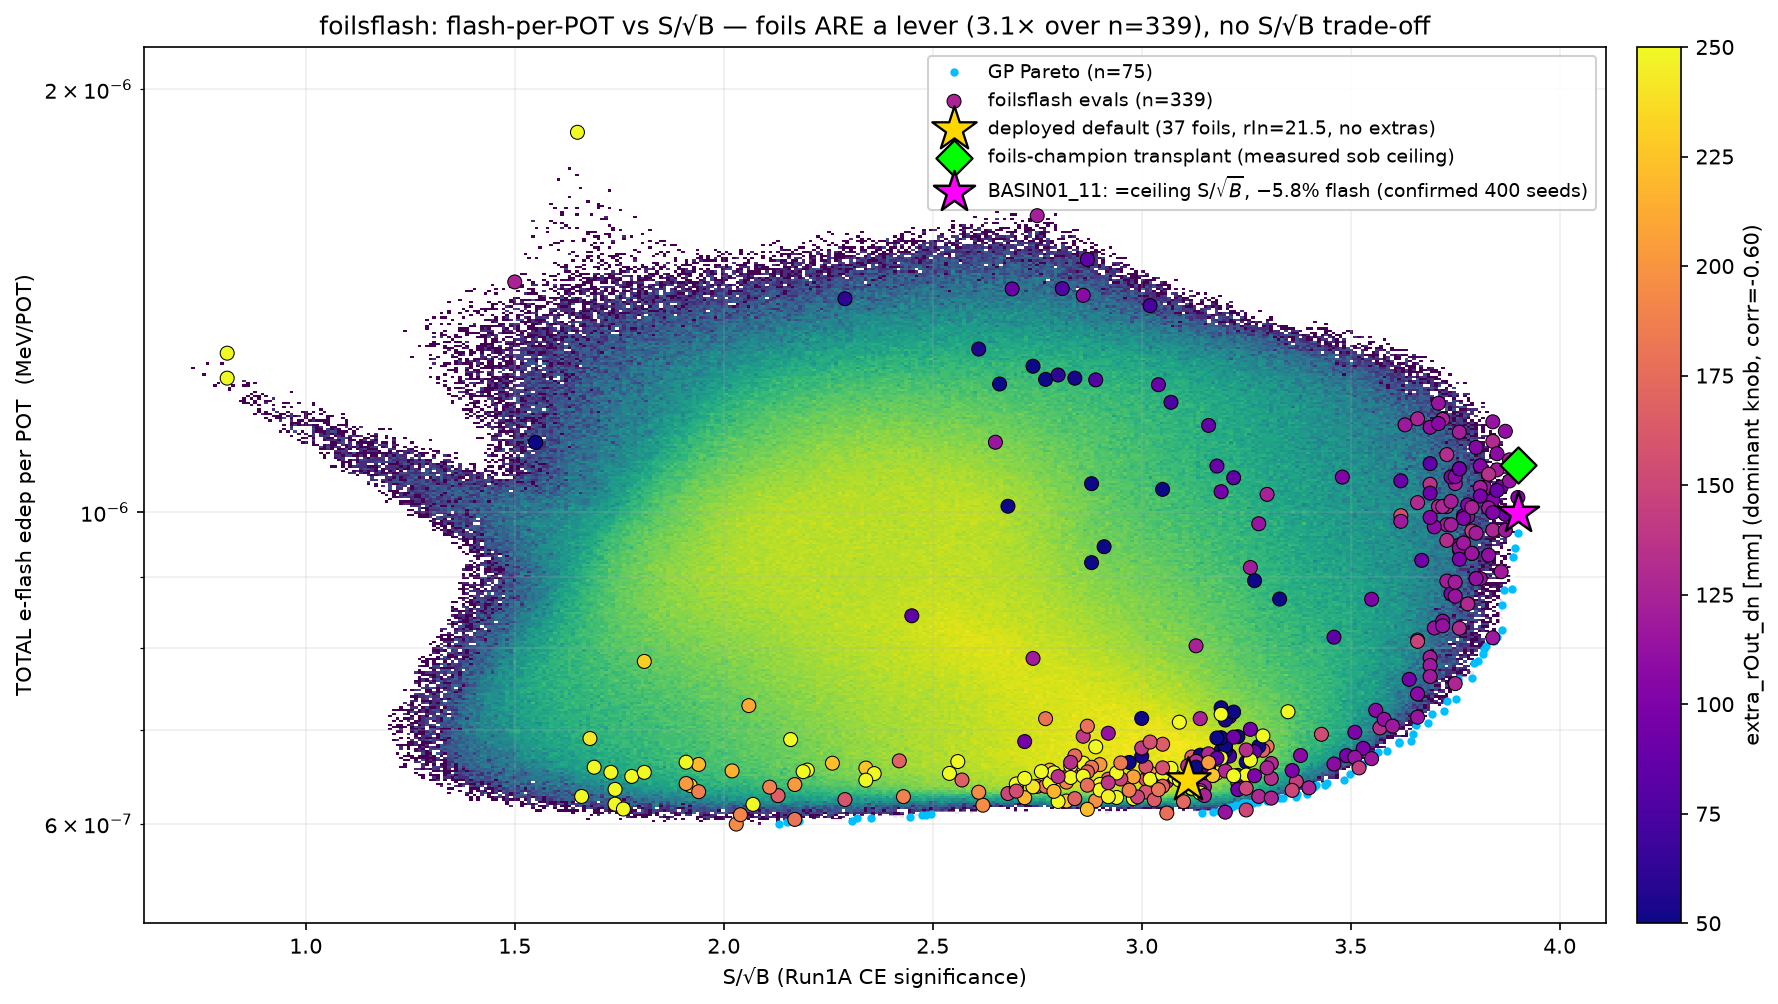
\includegraphics[height=0.70\textheight]{foilsflash_perpot_cloud_nochamp.png}
\end{center}
\footnotesize
339 evaluations. Gold star $=$ deployed default; green diamond $=$ the transplant S/$\sqrt{B}$
ceiling; \textbf{magenta star} $=$ \texttt{BASIN01\_11}: same 3.90 ceiling at \textbf{$-$5.8\%
flash} (400-seed confirmed). Colour $=$ downstream outer radius, the dominant knob. The cyan GP
Pareto front traces the reachable low-flash / high-S/$\sqrt{B}$ edge.
\end{frame}

\begin{frame}{The extra foils are a strong lever}
\begin{itemize}
  \item \textbf{3.1$\times$} spread in flash per POT across the explored geometry
        (GP fit $R^2 \approx 0.9$).
  \item More \textbf{upstream} material $\rightarrow$ \textbf{more} flash; larger
        \textbf{downstream} radius with bigger holes $\rightarrow$ \textbf{less}.
  \item S/$\sqrt{B}$ and flash are nearly uncorrelated ($-0.13$)
        $\rightarrow$ cutting flash is essentially \textbf{free} of signal.
\end{itemize}
\vspace{1.5em}
The foils act as a \textbf{scatterer of the on-axis electron beam} --- the same picture
behind Edmonds' central-hole result.
\end{frame}

\begin{frame}{Anatomy of the max-S/$\sqrt{B}$ point}
\begin{columns}
\begin{column}{0.42\textwidth}
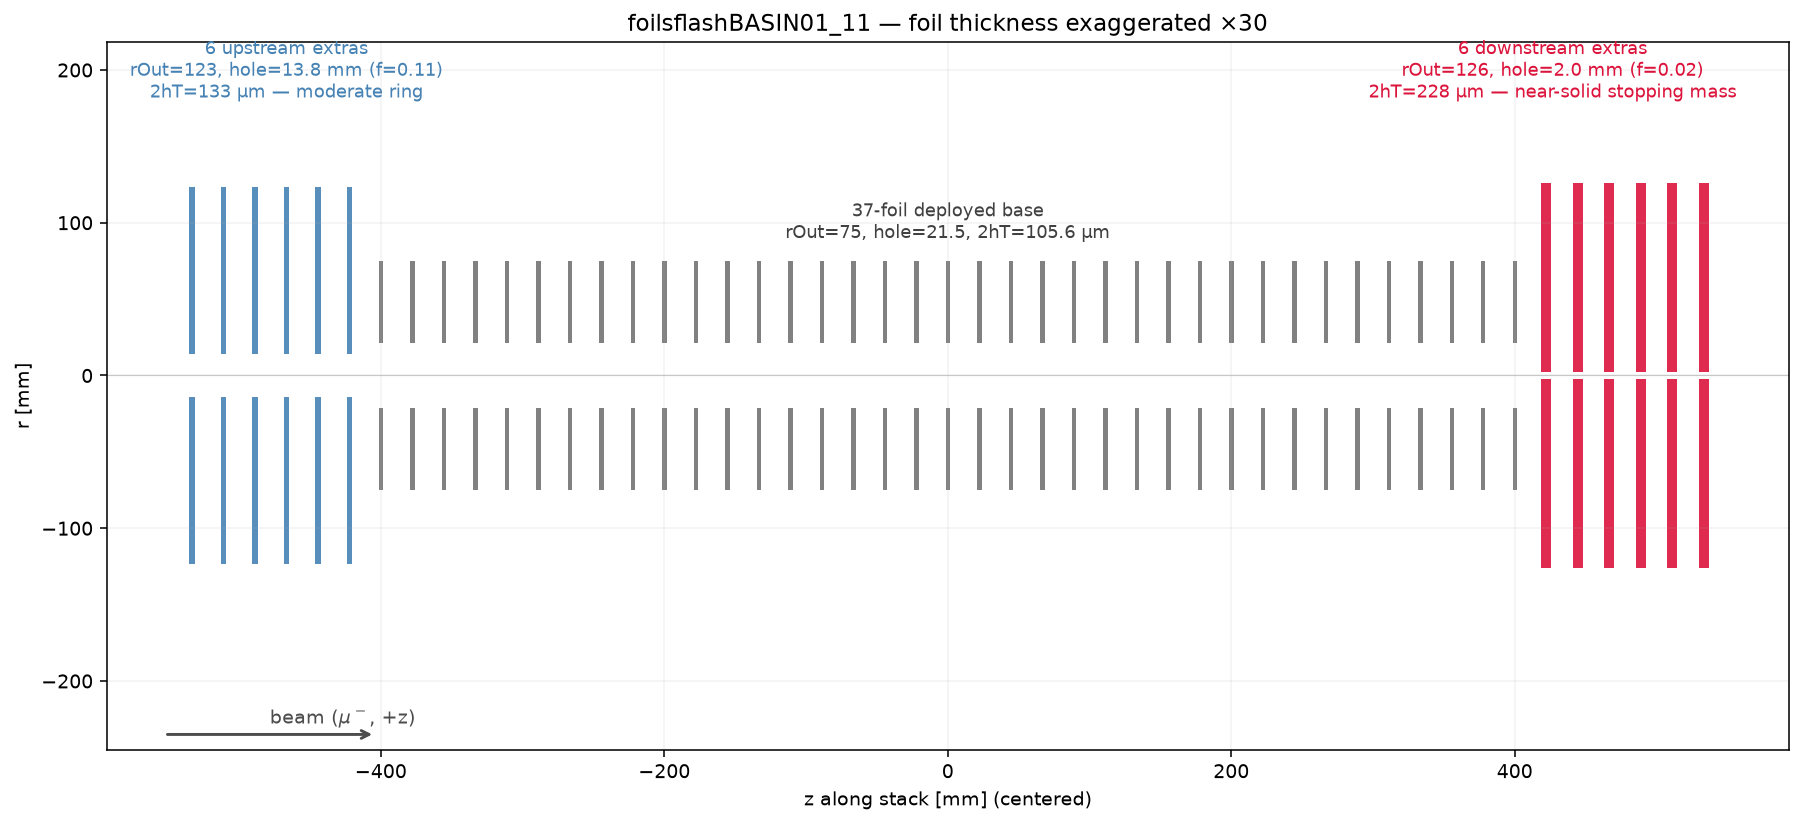
\includegraphics[width=\textwidth]{foilsflash_bestsob_sketch.png}
\end{column}
\begin{column}{0.58\textwidth}
\small
\begin{tabular}{lcc}
\toprule
design & S/$\sqrt{B}$ & flash [MeV/POT] \\
\midrule
\texttt{BASIN01\_11} (confirmed) & \textbf{3.90} & \textbf{1.00$\times10^{-6}$} \\
\texttt{SOBX01} (transplant)     & \textbf{3.90} & 1.08$\times10^{-6}$ \\
\texttt{ff14R01\_00} (exploit) & \textbf{3.84} & \textbf{8.14$\times10^{-7}$} \\
\texttt{ff11R00\_07} (champion)& 3.31 & \textbf{6.26$\times10^{-7}$} \\
deployed default               & 3.11 & 6.45$\times10^{-7}$ \\
\bottomrule
\end{tabular}
\end{column}
\end{columns}
\vspace{1em}
\footnotesize
Two routes to high S/$\sqrt{B}$: a thin \textbf{off-beam} ring, or thin \textbf{in-beam}
material that degrades the beam to stop more muons. A dense 20-point basin scan
\textbf{confirms 3.90 reproduces} and finds \texttt{BASIN01\_11} at the ceiling with
\textbf{$-$5.8\% flash} vs the transplant (400-seed re-eval: 1.00 vs 1.06$\times10^{-6}$,
$\sim$3.2$\sigma$). The flash floor itself is the \textbf{champion}, which beats deployed
on both axes.
\end{frame}

\begin{frame}{Top 10 configs by S/$\sqrt{B}$}
\scriptsize
Distinct geometries, replicates collapsed (flash averaged); 372 rows $\to$ 351 unique.
Flash in $10^{-6}$\,MeV/POT; \texttt{rOut}/\texttt{hT}/\texttt{rIn} in mm (up\,/\,dn); \texttt{rIn} $= f\cdot$\texttt{rOut} hole radius.
\vspace{0.4em}
\begin{center}
\begin{tabular}{@{}rlcccccl@{}}
\toprule
\# & config & S/$\sqrt{B}$ & flash & \texttt{rOut} & \texttt{hT} & \texttt{rIn} & \\
\midrule
1 & \texttt{BASIN01\_00} & 3.90 & 1.075 & 112/110 & 0.063/0.145 & 20.0/0.0 & transplant / ceiling \\
2 & \texttt{BASIN01\_16} & 3.90 & 1.024 & 110/103 & 0.052/0.144 & 24.9/5.8 &  \\
3 & \texttt{BASIN01\_11} & 3.90 & \textbf{0.999} & 123/126 & 0.066/0.114 & 13.8/2.0 & \textbf{confirmed op. point} \\
4 & \texttt{BASIN01\_03} & 3.88 & 1.053 & 113/114 & 0.090/0.136 & 23.2/0.1 &  \\
5 & \texttt{BASIN01\_17} & 3.88 & 1.090 & 111/122 & 0.076/0.148 & 12.1/1.5 &  \\
6 & \texttt{BASIN01\_04} & 3.87 & 1.142 & 91/112 & 0.044/0.177 & 9.5/3.7 &  \\
7 & \texttt{BASIN01\_14} & 3.87 & 0.997 & 118/95 & 0.038/0.108 & 15.2/1.3 &  \\
8 & \texttt{BASIN01\_09} & 3.86 & \textbf{0.971} & 104/117 & 0.024/0.123 & 26.6/4.1 & low-flash \\
9 & \texttt{18R01\_00} & 3.86 & \textbf{0.907} & 79/120 & 0.071/0.141 & 13.9/24.1 & holed dn \\
10 & \texttt{BASIN01\_02} & 3.86 & 1.042 & 131/98 & 0.045/0.162 & 31.7/2.2 &  \\
\midrule
--- & deployed (nominal) & 3.11 & 0.645 & --- & --- & --- & 37-foil base, no extras \\
\bottomrule
\end{tabular}
\end{center}
\vspace{0.4em}
\footnotesize
Rows 1--3 all sit at the \textbf{3.90 ceiling} --- \texttt{BASIN01\_11} owns it at the lowest flash.
Row 9 (\texttt{18R01\_00}) reaches \textbf{0.907} (downstream-holed) for only $-0.04$ in S/$\sqrt{B}$.
All top configs run above the \textbf{0.645} nominal --- the flash cost of the extra stopping mass
that lifts S/$\sqrt{B}$ from 3.11 to $\sim$3.9. BASIN01-heavy: that scan densely mapped the high-S/$\sqrt{B}$ basin.
\end{frame}

\begin{frame}{What the winning geometries share}
\small
The best-S/$\sqrt{B}$ configs converge on \textbf{compact foils with a nearly-solid downstream}
and a $\sim$deployed-size upstream hole --- these are \emph{stopping-target} foils, so more foil
mass stops more muons.
\vspace{0.3em}
\begin{center}
\begin{tabular}{@{}l c c l@{}}
\toprule
parameter & top-10 & median & \\
\midrule
\texttt{rIn\_dn} downstream hole & \textbf{4.5\,mm} & 48\,mm & \textbf{nearly solid} \\
\texttt{rIn\_up} upstream hole   & 19\,mm & 51\,mm & $\sim$deployed 21.5\,mm \\
\texttt{rOut} up / dn [mm]       & 109 / 112 & 142 / 125 & compact \\
\texttt{hT} up / dn [mm]         & 0.06 / 0.14 & 0.03 / 0.18 & moderate \\
\bottomrule
\end{tabular}
\end{center}
\vspace{0.2em}
\begin{itemize}\footnotesize
  \item \textbf{Every parameter correlates negatively with S/$\sqrt{B}$} --- solid, compact foils
        add stopping mass: corr \texttt{rIn\_dn} $-0.61$, \texttt{hT\_dn} $-0.57$, \texttt{rOut\_dn} $-0.50$.
  \item \textbf{The flash lever is the downstream geometry:} the downstream hole \texttt{rIn\_dn}
        (corr flash $-0.64$) and radius \texttt{rOut\_dn} ($-0.45$) cut flash --- and \emph{both also
        cut} S/$\sqrt{B}$. That single tension \textbf{is} the Pareto front.
  \item \textbf{\texttt{BASIN01\_11} threads it:} it opened a small downstream hole
        (\texttt{rIn\_dn} 2\,mm) and pushed \texttt{rOut\_dn} out (126 vs 110) --- the flash-reducing
        moves --- at a spot that \emph{kept} S/$\sqrt{B}$ at the 3.90 ceiling. Same sob, $-5.8\%$ flash.
\end{itemize}
\end{frame}

\begin{frame}{Central-hole A/B --- reproduces Edmonds}
Matched high-stats A/B: solid target vs a \textbf{21.5\,mm} central hole
($\sim$40\,M input $e^-$ each).
\vspace{1em}
\begin{center}
\begin{tabular}{lccc}
\toprule
observable & solid & holed & hole effect \\
\midrule
flash-event rate    & ---                  & ---                  & \textbf{$-24\%$} \\
total flash per POT & 8.2$\times10^{-7}$   & 6.4$\times10^{-7}$   & \textbf{$-21.5\%$} \\
\bottomrule
\end{tabular}
\end{center}
\vspace{1em}
\begin{itemize}\footnotesize
  \item Same direction and comparable magnitude to \textbf{Edmonds DocDB-10898}
        ($\sim$30\%) --- validates the flash pipeline end-to-end.
  \item The \textbf{deployed} Run1 target already carries this hole.
\end{itemize}
\end{frame}

\begin{frame}{Honest reading of the improvement}
\begin{itemize}
  \item \textbf{Flash: a tie at the floor, not a breakthrough.}
        Every ``better-flash'' point is $\le3\%$ below baseline --- within run-level noise.
        The deployed 21.5\,mm hole already sits at the flash floor.
  \vspace{0.5em}
  \item \textbf{S/$\sqrt{B}$: a real, resolved win.} Champion $+0.2$ ($\sim$20$\sigma$) at the
        same flash floor --- extra stopping mass buys more CE signal at no flash cost.
  \vspace{0.5em}
  \item \textbf{Caveat:} that gain carries un-modelled costs (added material, backgrounds this
        scan does not capture). Deploy-worthiness is a physics/cost call beyond the scan.
\end{itemize}
\end{frame}

\begin{frame}{Conclusion \& next steps}
\begin{itemize}
  \item Stopping-target foils are a \textbf{usable electron-flash lever}: $\approx$3.1$\times$
        swing in tracker flash per POT with \textbf{no S/$\sqrt{B}$ trade-off}.
  \vspace{0.5em}
  \item The \textbf{champion} beats the deployed target on both axes, and the S/$\sqrt{B}$
        ceiling is measured and priced --- \textbf{3.84 at $+26\%$} flash.
  \vspace{0.5em}
  \item The central-hole A/B \textbf{reproduces Edmonds}, confirming the flash pipeline is
        physically sound.
  \vspace{0.5em}
  \item \textbf{Next:} the central-hole line (\texttt{bo-foilshole}) --- Edmonds' $\sim$30\%
        central-hole lever is an order of magnitude larger than the outer envelope bought.
\end{itemize}
\end{frame}

\end{document}
